\documentclass[twocolumn,a4paper]{article}

\usepackage{t1enc}          % this is needed if one likes to put some
\usepackage[utf8]{inputenc} % special characters (umlauts, Polish ę,ą, etc) in the text

\usepackage{amsfonts}

\usepackage{pe}           % possible options: polish, proceedings
                          % polish mode will switch to Polish language (Fig. -> Rys., etc)
                          % proceedings mode will not display the footer


\peNo{R. 86 NR 1/2010}    % year and number of the journal -- will be used in the page footer
                          % meaningless in proceedings mode

\startpage{91}            % first page number


% put local definitions here
\def\baselinestretch{1}   % setting it to 0.99-0.98 allows us to pack more content
                          % in limited number of pages (this is not welcome be the Editor ;-)
\def\tabcolsep{3.0pt}     % tables are a little bit narrower

%\authorheading{Author}   % use (uncomment) it if there is only one author
                          % - to redefine header of the author data at the end of paper

\def\vect#1{\text{\bf #1}}
\def\rref#1{\figurename~\ref{#1}}
% end of local definitions

% before-text material

\title{Searching for the best optimizer for an automated CAD system}

\author{Jacek STARZYŃSKI\aff1, Robert SZMURŁO\aff1, Piotr ROWIŃSKI\aff1, Andrzej MICHALSKI\aff{1,2}\\
Zbigniew WATRAL\aff2, Stanisław WINCENCIAK\aff1}

\affiliation{Warsaw University of Technology (1), Military Academy of Technology (2)}


\abstract{
Choice of a robust and universal optimization procedure is one of the crucial design decision for many Computer Aided Design systems. Evolutionary Algorithms are commonly advised in such situations. This paper shows, that such choice is not always the best one. Use of a classical deterministic procedure may lead to better results which are obtained much faster. Example CAD system for electromagnetic flow meters design is used as a practical example illustrating the problem.
}

\streszczenie{
Komputerowe systemy wspomagające projektowanie wymagają od swoich twórców wyboru właściwej: uniwersalnej i odpornej na błędy użytkownika, procedury optymalizacji. Często proponowanym rozwiązaniem jest wykorzystanie w takich systemach algorytmów ewolucyjnych. W tym artykule próbujemy pokazać, że taki wybór nie zawsze jest właściwy. Zastosowanie klasycznego algorytmu deterministycznego prowadzi bowiem do lepszego rozwiązania, które ponadto jest znajdowane znacznie szybciej. Rozważania zostały zilustrowane przykładem systemu wspomagającego projektowanie przepływomierzy elektromagnetycznych.
\textbf{(Wybór procedury optymalizacyjnej dla systemu CAD)}
}

\slowakluczowe{systemy CAD, optymalizacja, algorytmy deterministyczne, algorytmy ewolucyjne}


\keywords{CAD, optimal design, deterministic algorithms, evolutionary algorithms}


\begin{document}


\maketitle


\section{Introduction}
Automated Computer Aided Design (CAD) systems are currently commonly used in many areas of engineering. Use of such tools allows to design and prototype final products with better performance more effectively. One of the crucial components of many CAD systems is an automated optimization procedure. We assume here, that the user of such a system is responsible for general design decisions, and the system's role is to find the best parameters for the chosen design.  Such tasks are usually formulated in form of one or many cost functions and the best values are found in process of minimization of these functions.
 Nowadays the most common choice of cost function minimizer
is one of the stochastic algorithms. Such methods are simple to implement, they search for globally best solution and
they may be applied for practically any cost function: even discontinuous and multimodal.

Here we shall present a case study of process of selecting such minimizer for an example CAD system.
The stochastic optimizer will be compared to the deterministic one in terms of the simplicity, robustness, quality of the results and speed.



\section{Example CAD system}

In the paper we use a CAD system for electromagnetic flow meter (EFM) design as an illustrative example. In the EFM externally induced magnetic field $\vect{B}$ acts on a moving conducting liquid and creates creating electric field $\vect{E}$ which can be measured as a potential difference on the electrodes \textbf{e$_\text1$-e$_\text2$} situated on the banks (see~\rref{fig1}).
\begin{figure}[htb]
\begin{center}
 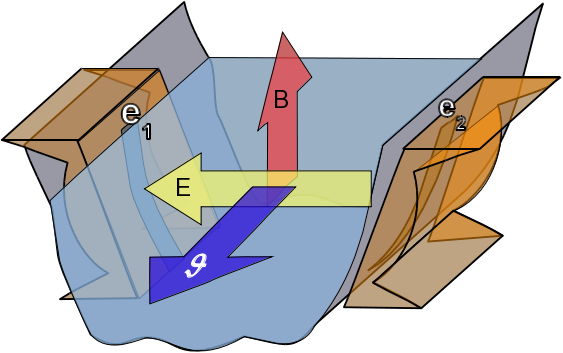
\includegraphics[width=0.57\linewidth]{img/flow1a.png}
 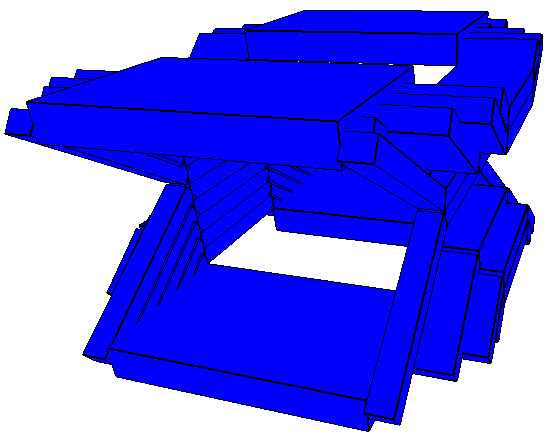
\includegraphics[width=0.42\linewidth]{img/cewka_nizsza.png}
 \caption{An electromagnetic flow meter: principle of operation (left) and sample shape of the coil (right)}
 \label{fig1}
 \end{center}
\end{figure}
It can be shown, that for the proper distribution of the magnetic field $\vect{B}$ (for example uniform perpendicular component) the signal can be made proportional to the total
flow~\cite{IEEETM98fm}. Thus the optimal design of the EFM is usually formulated as a search for the coil shape.

A dedicated CAD system---Flow Meter Design Tool (FMDT)~\cite{IEEEInstrMeas2009} is aimed at helping to design and test EFM prototypes.
A designer can use FMDT to manage several alternative projects, design and optimize coil shapes and test their performance by numerical simulation.

From our perspective the most interesting part of the FMDT is the \textit{coil designer}. It can be
divided into two components: the \textit{pre-designer} which helps to propose starting topology of the coil, and the \textit{optimizer} which controls 
the optimization routine to calculate the best dimensions for the proposed topology.

To explain the optimization task it is necessary to present how the coil is described in FMDT. Figure~\ref{fig1} presents a 3D view
of the optimized coil.
It can be noticed that the main, working part of the coil is formed of rectangular blocks. This assumption comes from
the technological requirements for realization of the designed shape. The designer selects a basic topology, number of sections, initial lengths and widths of sections.
The initial coil may be evaluated with field simulation to check the magnetic field strength and predict signals for preselected
flow(s).

\section{The optimization task}


The following design parameters were used in experiments: widths of all sections, length of the working part, total depth of the coil and shape (width or height) of the side-to-side connections. The objective function can be defined in several ways~\cite{IEEEIM2002}. We have used a postulate of uniform distribution of the vertical component of magnetic flux density. Thus the cost function is defined as
\begin{equation}
 f(\mathbf d) = \frac{1}{N}\sqrt{ \sum_N ( B_{y,i} - \bar B )^2 },
\end{equation}
where $\mathbf d$ is a vector of the design parameters, $N$ is the number of control points within the channel, $B_{y,i}$ is the vertical component of  magnetic flux density at the $i$-th node and $\bar B$ is the desired value of $B_y$. The control points are spread on an uniform lattice grid in the channel.

For experiments analyzed in this paper we have designed a coil for rectangular channel 15 centimeters wide and 11 cm deep. We have assumed, that the controlled part of the channel is 5 cm long. The internal width of the coil was 16 cm. The working part of the coil contained 20 blocks and working parts were connected above and below the channel. The initial width of all blocks was 1 cm. Current density was set to 1e6 A/m$^2$.

Results of the magnetic field simulation for the initial coil shape is shown in~\rref{fig5}. The absolute value of $B_y$ is in the range of 3.89 mT to 7.223 mT. After optimization process we would like to obtain possible uniform field close to 7 mT.

\begin{figure}[htb]
\begin{center}
 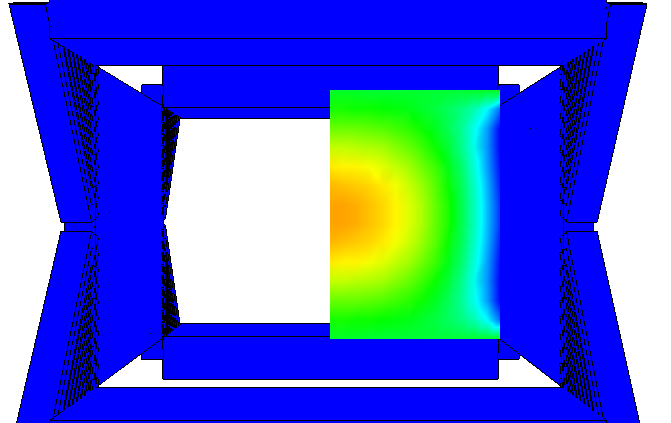
\includegraphics[width=0.9\linewidth]{img/initial_field-kadr.png}
 \caption{Initial coil (3D view) and $B_y$ distribution at the central cross-section of the channel}
 \label{fig5}
 \end{center}
\end{figure}

We have used test problems with the same initial coils, but slightly different constraints. We have started with the initial coil, presented above, and allowed
to change the shape and the total length of the coil. This resulted in 21 design variables: 20 representing the widths of sections and the last one representing the length of the working part of the coil.
In the first problem (Problem A) the widths were allowed to change in range of 1 mm to 3 cm, in the second one (Problem B) the upper bound was extended to 5 cm. Constraints of the coil length were the same: from 5.01 to 15 cm.

\section{Experiments with Levenberg-Marquardt algorithm}

The deterministic Levenberg-Marquardt (LM) optimizer, which was used in FMDT, was implemented with help of the public domain library \texttt{levmar}~\cite{lourakis04LM}.
The Jacobian of the cost function was calculated numerically. Two examples of optimized shapes are shown in~\rref{fig6}.

\begin{figure}[htb]
\begin{center}
\begin{tabular}{m{.48\columnwidth}m{.48\columnwidth}}
 \centering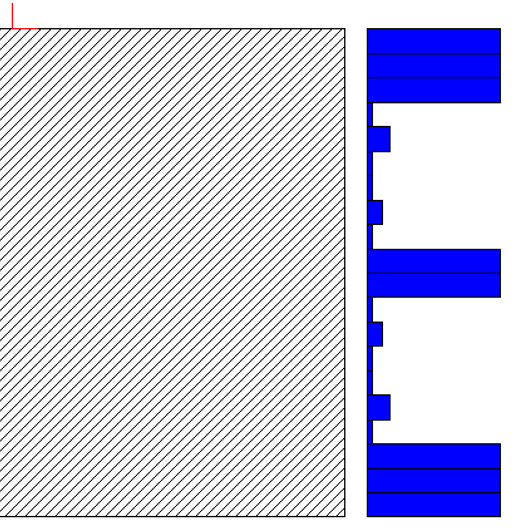
\includegraphics[height=0.35\columnwidth]{img/LMOpt_coil_0p03.png} &
 \centering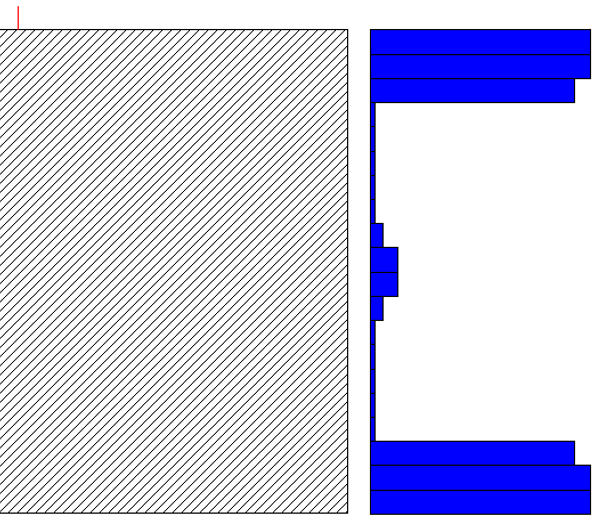
\includegraphics[height=0.35\columnwidth]{img/LMOpt_coil_0p05.png}
\end{tabular}
 \caption{The results of the deterministic optimization: solution of Problem A on the left side, Problem B on the right side}
 \label{fig6}
 \end{center}
\end{figure}

Experiments with different starting points (initial shape of the coil) are illustrated in~\rref{fig7}. It may be noticed, that differences in the coil shape are minor, and the resulting field distributions are as well very similar. In our opinion this variation originates from numerical calculation of the Jacobian.

\begin{figure}[htb]
\begin{center}
 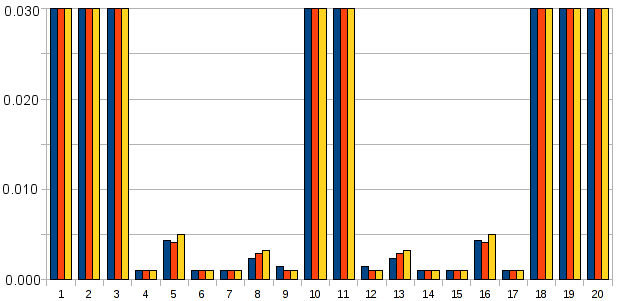
\includegraphics[width=0.95\linewidth]{img/por_cewek3a.png}
 \caption{Comparison of results of LM optimizer for Problem A with different starting points: blue -- algorithm started from upper bound, orange -- from the lower bound, yellow -- from the midpoint of lower and upper bounds}
 \label{fig7}
 \end{center}
\end{figure}

Giving more freedom to the optimizer in the Problem B resulted in a different coil shape (presented in the right side of~\rref{fig6}) and better (more uniform) distribution of $\vect{B}$. Changes of the starting point resulted in small changes of the optimal shape. The effect is similar to the on which is presented in~\rref{fig7}.


\section{Experiments with genetic algorithms}
The base for the genetic algorithm optimizer was the open source library \texttt{GAlib}~\cite{GAlib} which contains a set of C++ ``genetic'' objects. On the basis of these objects the typical genetic algorithms was implemented.
We have used real coding, roulette wheel selection method and elitism to preserve the best solution found. We have tested generational, steady-state algorithms and deterministic crowding niching. On the basis of all conducted experiments (few hundreds of optimizations) we are not able to say, which version of GA performs best.

We have experimented with different parameters of the GA algorithm. It was quite obvious, that the size of population can not be small for 21 design variables. For practical reasons we wanted to keep acceptable (less than 1 hour) time of solution. This set upper limits for the size of population and the numbers of generations. In~\rref{fig8} the results of two example experiments are presented. Both results were obtained in 100 generations of 400-individuals population.
\begin{figure}[htb]
\begin{center}
\begin{tabular}{m{.48\columnwidth}m{.48\columnwidth}}
 \centering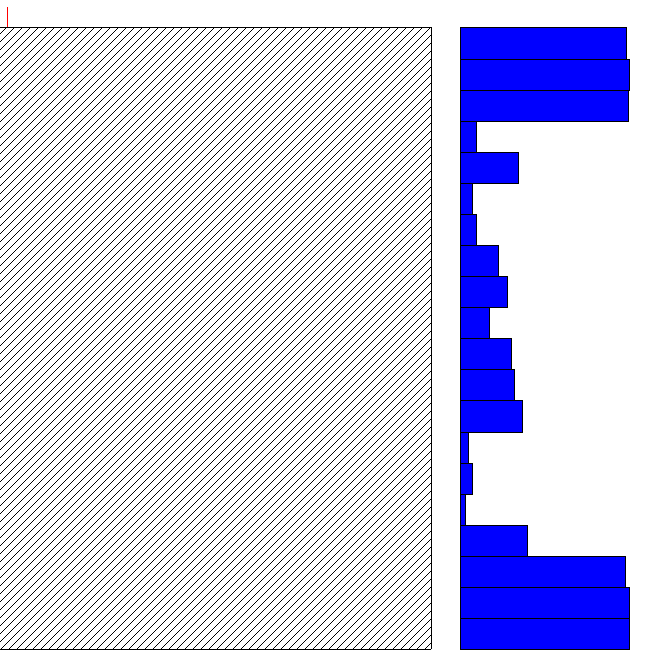
\includegraphics[height=0.35\columnwidth]{img/GAOpt_coil_0p03.png} &
 \centering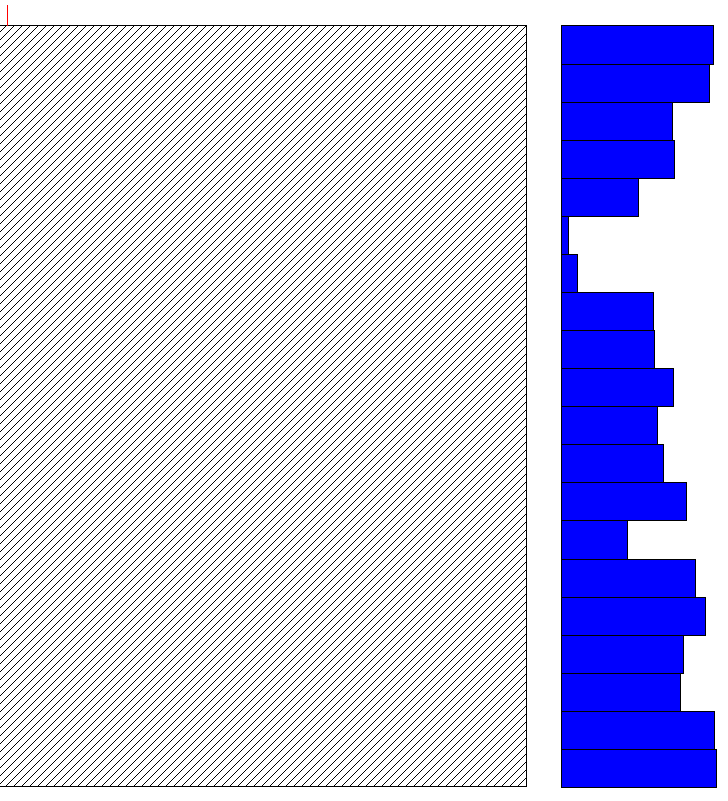
\includegraphics[height=0.35\columnwidth]{img/GAOpt_coil_0p05.png}
\end{tabular}
 \caption{The results of the genetic optimization of Problem A (left) and Problem B (right)}
 \label{fig8}
 \end{center}
\end{figure}

Comparison~\rref{fig6} and~\rref{fig8} shows clearly, that the genetic optimizer produces much worse results than the deterministic one. All shapes obtained with the genetic algorithm are less smooth and asymmetric. Change
of the GA parameters usually leads to a different final result. The GA results differ much more than solutions obtained with multistart technique by the Levenberg-Marquardt optimizer. Is can be seen in~\rref{fig9} where the results of three different runs of GA solving the Problem A are compared.
\begin{figure}[htb]
\begin{center}
 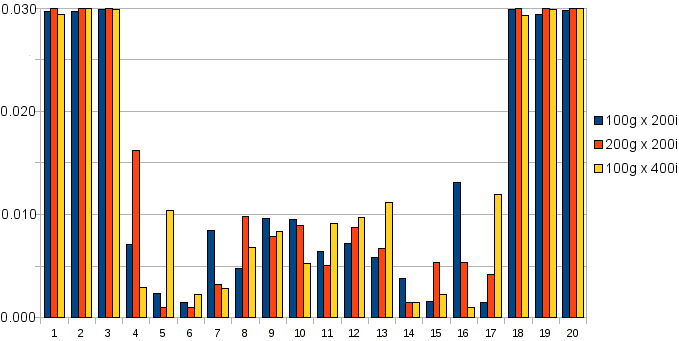
\includegraphics[width=0.999\linewidth]{img/por_cewek3_GA.png}
 \caption{Comparison of the results of GA optimizer for Problem A and different GA parameters: : blue -- 100 generations of 200 individuals, orange -- 200 generations of 200 individuals, yellow -- 100 generations of 400 individuals}
 \label{fig9}
 \end{center}
\end{figure}
One can notice that while width of the upper and lower coil blocks stick to the constrains (what is similar to the results
obtained with the LM optimizer), the widths of blocks in the inner part of the coil differ quite substantially.
The final result can be improved by using more generations of bigger populations, but time of computations is then unbearable. The influence of the population size and number of generations on the quality of the final result is not obvious and
it is very difficult to propose the minimal values which will guarantee satisfactory results of optimization.
To illustrate this behavior one can study the results presented in~\rref{fig10}.
\begin{figure}[htb]
\begin{center}
 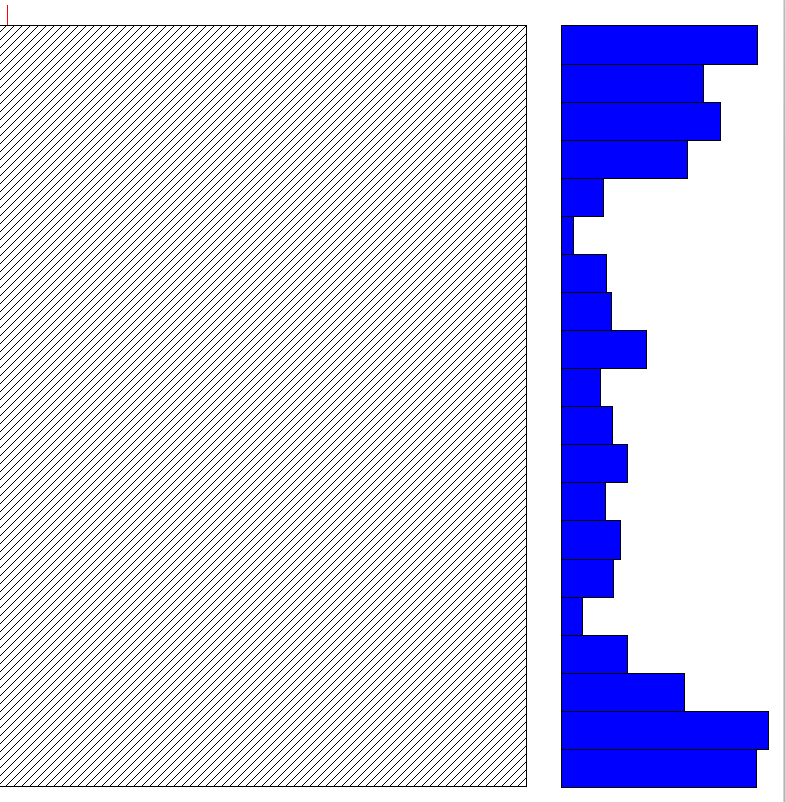
\includegraphics[width=0.32\linewidth]{img/GAOpt_1mm-3cm_50g200i.png}
 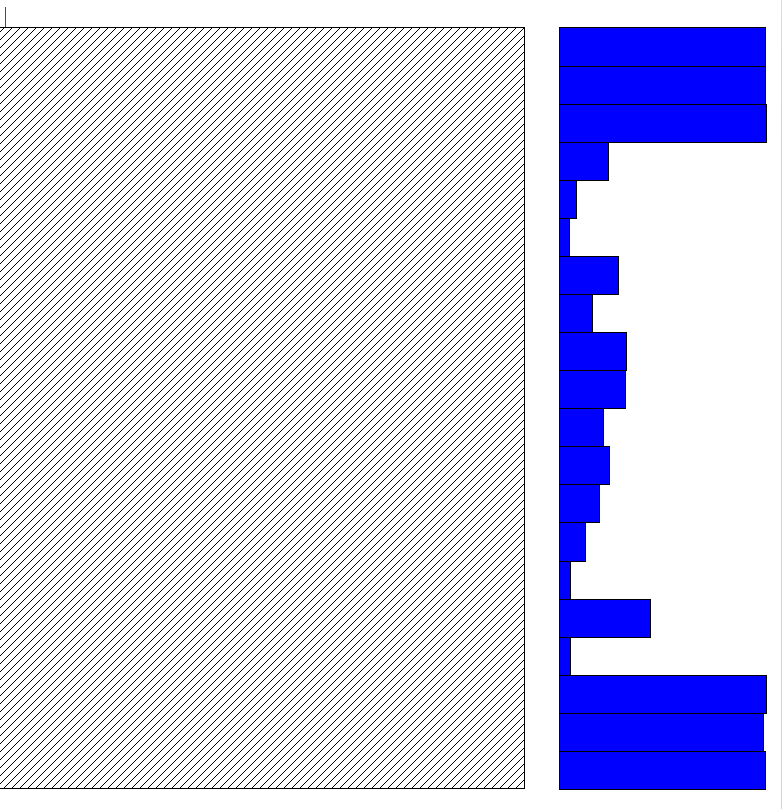
\includegraphics[width=0.32\linewidth]{img/GAOpt_1mm-3cm_100g200i.png}
 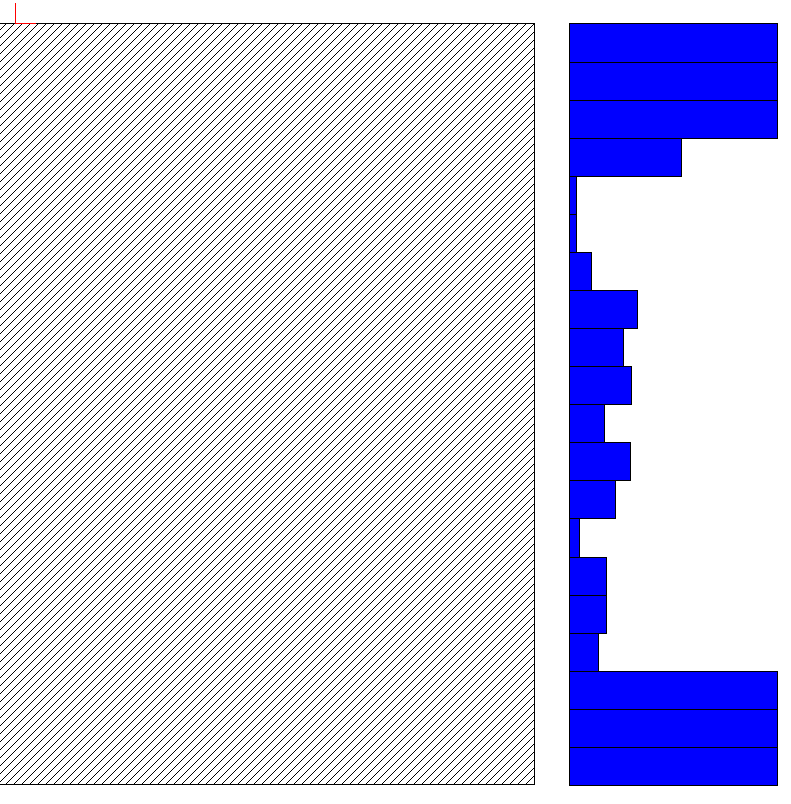
\includegraphics[width=0.32\linewidth]{img/GAOpt_1mm-3cm_200g200i.png}
 \caption{Comparison of the best Problem A coil shapes obtained with the GA optimizer for different number of generations and same size of populations. From left to right: 200 individual population running for 50, 100, 200 generations}
 \label{fig10}
 \end{center}
\end{figure}
It is quite obvious than the result obtained with 50 generations of 200-individual population is the worst one, but comparison
between the results obtained with 100 and 200 generations is not simple at all. We shall compare them using field histograms, showing what proportion  of the channel space is covered with the selected values of magnetic flux density. Such histograms for both discussed solutions are presented in~\rref{fig11}.

\begin{figure}[bth]
\begin{center}
 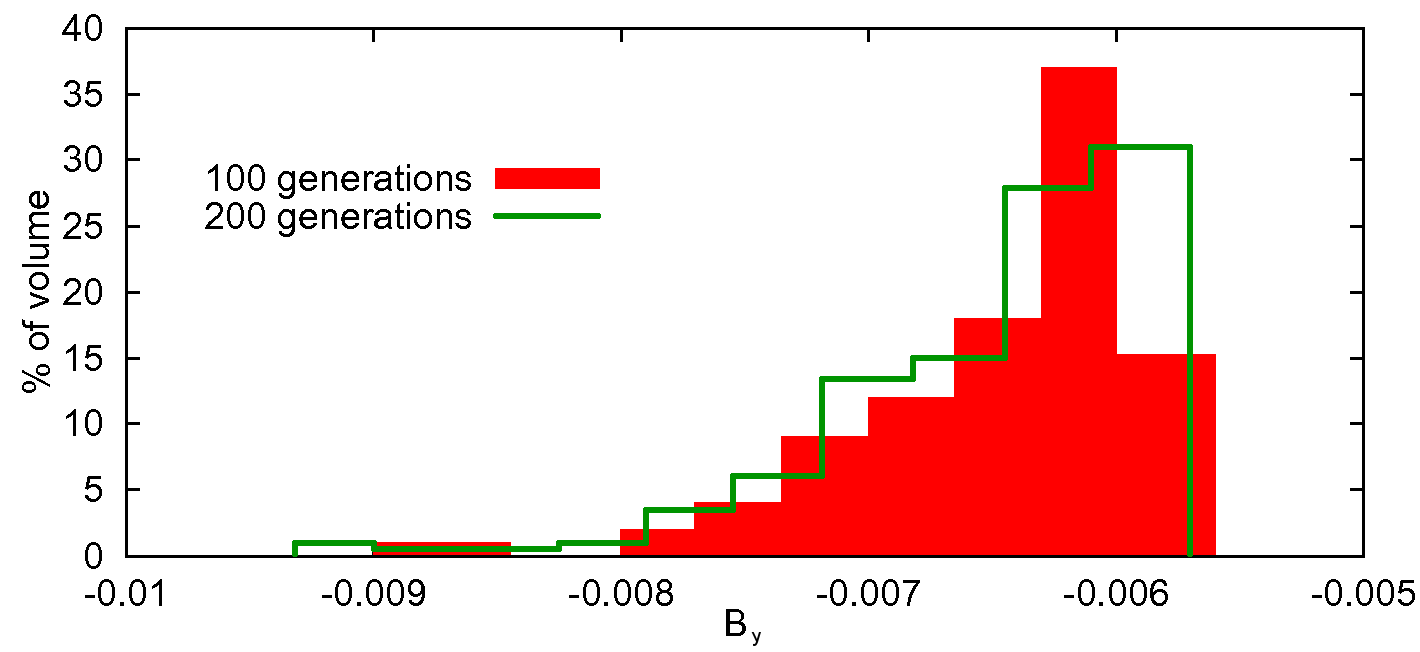
\includegraphics[width=0.99999\linewidth]{img/hisGA200i.png}
% \includegraphics[width=0.95\linewidth]{img/his100gx200i.png}
% \includegraphics[width=0.95\linewidth]{img/his200gx200i.png}
 \caption{Comparison of the field histograms for the best coils obtained with the GA optimizer for different number of generations and same size of population (200 individuals)}
 \label{fig11}
 \end{center}
\end{figure}

The good histogram should: a) be possibly narrow and b) exhibit the maximum for the flux density close to the desired value. For the desired value of $B_y$set to 7 mT the solution obtained with 200 generations could eventually be chosen as the better one, but it is not obvious at all.

\balance

\section{Quality of the results}
For comparison to the results presented in~\rref{fig11} let us show the field histograms for the best coils found by the
deterministic optimizer, shown in~\rref{fig12}. Comparing these histograms with those in~\rref{fig11} we can see that the coil found with the LM optimizer is better.

\begin{figure}[htb]
\begin{center}
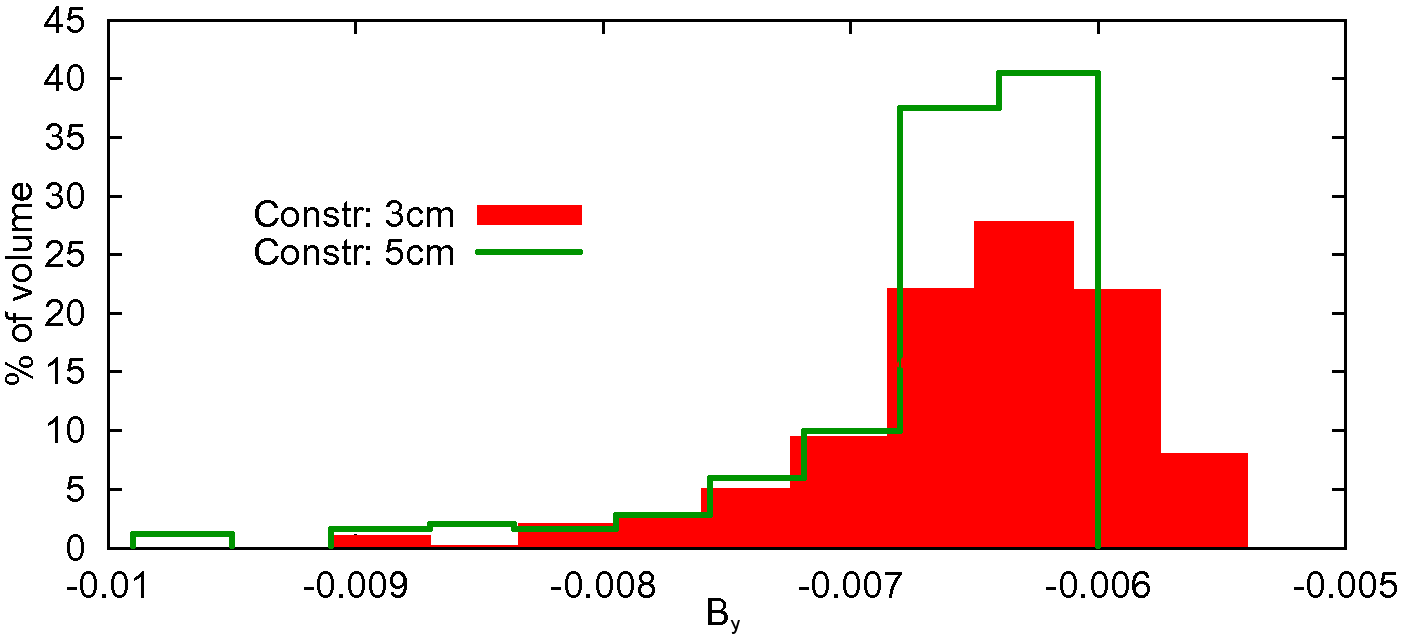
\includegraphics[width=0.99999\linewidth]{img/hisLM_por.png}
% \includegraphics[width=0.975\linewidth]{img/hisLM.png}
% \includegraphics[width=0.975\linewidth]{img/hisLM_5cm.png}
 \caption{Field histograms for the best coils obtained with the LM optimizer}
 \label{fig12}
 \end{center}
\end{figure}

\hphantom.
\bigskip
Histograms presented in~\rref{fig12} confirm that Problem B, with more loose constrains, allows us to
find a coil which generates better field. As it could be expected, this better coil will be also more
expensive in terms of production and application. Figure~\ref{fig6} shows that this coil needs more wire
turns what causes more material and more feeding power.


\section{Conclusion}

Optimal design problem formulated in terms of a cost function may be solved by a deterministic or by a stochastic algorithm. The former approach is usually faster, but it requires continuous, differentiable cost function and it can converge to a local minimum. Stochastic algorithms in theory search for the global minimum and are much more tolerant. The minimized cost
function may be multimodal and discontinuous. However, the biggest disadvantage of stochastic algorithms is their computational burden. In practice they require thousands of cost-function evaluations what makes them practically slow, comparing to deterministic methods.
Speed-up of such algorithms can be obtained by reduction of the population size or number of generations, but this can seriously
decrease the quality of obtained results.

The practical example presented in this paper suggests that application of the deterministic optimizer should be always considered. If the cost function is differentiable and its gradient may be calculated numerically then the implementation
of the deterministic optimizer is not more difficult then the implementation of the evolutionary one. Moreover the
optimal design will be obtained much faster with the deterministic optimizer and its quality will be much better.

Usually much more programming effort is needed if one wants to calculate the more exact (analytical) values of the gradient
or the Hessian matrix, but the quality of the results obtained with such implementation should be superior.

Comparison of two example desing problems (A and B) and their solutions suggests that the optimality criterion should be
forced not only by the field quality, but also by some additional criteria: costs of production and exploatation of the device.
This, however, needs different, multiobjective approach to the optimal design.

\begin{thebibliography}{999}
\let\titem\relax % bez wyrozniania tytulow ksiazek

\bibitem{IEEETM98fm}
Michalski A., Starzyński J., Wincenciak S.:
\newblock Optimal design of the coils of the electromagnetic flow meter,
\newblock {\titem IEEE Transactions on Magnetics}, 34(5), pp.~2563--2566, Sep.
  1998.

\bibitem{IEEEIM2002}
Michalski A., Starzyński J., Wincenciak S.:
\newblock 3D Approach to Design the Excitation Coil of an Electromagnetic Flow Meter,
\newblock {\titem IEEE Trans. Instrumentation and Measurement},  51(4), pp.~833--839, 2002.

\bibitem{IEEEInstrMeas2009}
Starzyński J., Szmurło R., Michalski A.:
\newblock Computer-Aided Design Tool for Electromagnetic Sensors,
\newblock {\titem IEEE Instrumentation and Measurement Magazine}, 12(3), pp.~28-33, Jun.
  2009.

\bibitem{lourakis04LM}
M.I.A. Lourakis.
\newblock levmar: Levenberg-marquardt nonlinear least squares algorithms in
  {C}/{C}++.
\newblock [web page] \verb+http://www.ics.forth.gr/~lourakis/levmar/+, Jul.
  2004, Apr. 2009.
\newblock [Accessed on 31 Jun. 2009.].

\bibitem{GAlib}
Matthew Wall,
\newblock GAlib A C++ Library of Genetic Algorithm Components
\newblock [web page] \verb+http://lancet.mit.edu/ga/+.
\newblock [Accessed on 31 Jun. 2009.].

\end{thebibliography}


\authordata{
Ph.D. Jacek Starzyński, Ph.D. Robert Szmurło, M. Sc. Piotr Rowiński, Prof. A. Michalski, Prof. S. Wincenciak,
Institute of Theory of Electrical Engineering,
Measurement and Information Systems,
Faculty of Electrical Engineering,
Warsaw University of Technology,
ul. Koszykowa 75,
00-662 Warszawa, Poland,
email: \underline{jstar@iem.pw.edu.pl},
Prof. A. Michalski, Ph.D. Zbigniew Watral, Institute of Electronic Systems,
Military Academy of Technology, ul. Kaliskiego 2, 00-489 Warszawa, Poland, email: \underline{zwatral@wel.wat.edu.pl}}

\end{document}

